\documentclass[12pt]{article}

% This is LaTeX template for AA2 Final Project Report
% Figure package
\usepackage{graphicx} %extension of graphics package
\usepackage{subcaption}
% \usepackage[draft]{graphicx} %edge only
% Directory latex
\graphicspath{{./images/}}

\usepackage[italian]{babel}
\usepackage[babel]{csquotes}
\usepackage[style=numeric,backend=biber]{biblatex}
\bibliography{biblio.bib} 
\usepackage{url}
\usepackage{pdflscape}
\usepackage{hyperref}
\usepackage[usenames,dvipsnames,svgnames,table]{xcolor}
\usepackage{amssymb}%for real symbol. It seems isnt include in amsmath package LOL
\usepackage{mathtools}
\setlength{\parindent}{1in}
\setlength{\parskip}{12pt}
\usepackage{listings}
\usepackage{caption}
\lstset{
basicstyle=\small\ttfamily,
keywordstyle=\color{MidnightBlue}\bfseries,
identifierstyle=\color{Black},
commentstyle=\color{Green}\itshape,
stringstyle=\color{Red}\ttfamily,
showstringspaces=false,
%numbers=left, numberstyle=\tiny,
%stepnumber=1, numbersep=10pt,
tabsize=4,
framexleftmargin=5mm, rulesepcolor=\color{Gray},
frame=tb,
backgroundcolor=\color{LightGray},
language={Java},
%mathescape=true,
%fontadjust=true,
%breaklines=true,breakatwhitespace=true,breakautoindent
}
\renewcommand\lstlistingname{Codice}
\setcounter{secnumdepth}{4}

\begin{document}
\renewcommand{\figurename}{Fig.}
\begin{center}
\LARGE\textbf{Stream Video Processor\\Implementazione per architetture multi-core mediante l'utilizzo delle librerie FastFlow e Threads C++11}\\
\vspace{0.2in}
\center
\normalsize{Maurizio Idini}\\
\normalsize{maurizio.idini [at] gmail.com}\\
\normalsize{SPM Final Project (A.A. 2015-16)} \\
\normalsize{\today}\\
\end{center}

\section*{Abstract}
In questa relazione si analizza la risoluzione e l'implementazione sequenziale e parallela del problema del \textbf{Stream Video Processor} affrontando, come caso d'uso, il problema del Reducing Video Size, ossia dato un video, si riduce la grandezza di ogni frame secondo un dato parametro, lavorando su architetture a pi\`u cores. L'implementazione parallela \`e stata attuata mediante l'utilizzo della libreria \textbf{FastFlow} e della libreria standard \textbf{Thread C++11}. Si son confrontate poi le prestazioni fra loro e con i modelli teorici.

\section{Introduzione}
Un file video, generalmente di formato .avi, pu\`o essere descritto come una sequenza di frames, ossia matrici codificate in un determinato modo. Generamente, la codifica pi\`u comune definisce ogni pixel del frame come una tupla di t valori, corrispondente ai canali di codifica del frame, come RGB o HSV, e che dunque rappresentano il colore del pixel. Ad esempio, OpenCv codifica generalmente i frames mediante la macro \texttt{CV\_8UC3}, dove 8 sono i bits che rappresentano il valore, U denota che il valore \`e Unsigned, e dunque il valore \`e espresso nel range [0,255], 3 denota il numero di canali. Ad esempio, un elemento di un frame, ossia un'immagine definita da una matrice (che in OpenCV \`e rappresentata dall'oggetto Mat),  \`e una terna [12,136,200].

\\Operare dunque su un file video significa operare su ogni singolo frame un'operazione (conforme), ossia 
% Il problema del \textbf{Reducing Video Size} si pu\`o riassumere nelle seguenti fasi:
\begin{itemize}
\item accedere al video in input e creare un nuovo video in output
\item accedere ad ogni singolo frame del video in input
\item applicare un'operazione al frame corrente
\item scrivere il frame risultante nel nuovo video
\end{itemize}
% \item applicare  alle stesse
Dunque l'operazione da applicare al frame pu\`o generalmente essere un filtro \texttt{Blur}\footnote{\url{http://docs.opencv.org/3.1.0/da/d54/group__imgproc__transform.html#gsc.tab=0}}, un \texttt{Thresold}, una \texttt{Resize} della dimensione del video, o qualsiasi altra operazione, seppur ammissibile.
\\In questo progetto si \`e scelto di applicare la \texttt{cv::resize}\footnote{\url{http://docs.opencv.org/3.0.0/da/d54/group__imgproc__transform.html#ga47a974309e9102f5f08231edc7e7529d}} come operazione sui frames. Pi\`u avanti si formalizzer\`a il problema con pi\`u precisione.
\\Le implementazioni proposte sono realizzate in C++11, in particolare quelle parallele lavorano mediante la libreria \textbf{FastFlow}\footnote{\url{http://calvados.di.unipi.it/}} e la libreria standard \textbf{Thread C++11}\footnote{\url{http://www.cplusplus.com/reference/thread/thread/}}. Ogni implementazione utilizza la libreria \textbf{OpenCV}\footnote{\url{http://www.opencv.org}} per operare su video e immagini.

\\ \textbf{FastFlow} \`e un C++ parallel programming framework, supporta stream e data parallelism e la dichiarazione ed istanziazione degli skeleton \`e molto semplice ed immediata, il che permette di scrivere poco codice non funzionale e concentrare il lavoro su quello funzionale. 

\\La \textbf{Standard-Library Thread} \`e il nuovo supporto alla programmazione Multi-Threading offerta da C++11; tale libreria si appoggia alla nota \texttt{Pthread}, ma risulta molto pi\`u chiara e user-friendly. 

\\L'implementazione parallela risulta molto differente utilizzando queste due librerie: da un lato, si ha la possibilit\`a di concentrarsi sul codice funzionale, per assurdo quasi trascurando come avviene il parallelismo o come la libreria condivida, invia e processa i dati, e questo \`e il caso di FastFlow. Dall'altro lato, quasi non si distingue pi\`u fra codice funzionale e codice non funzionale, e questo \`e il caso di Thread C++11.

\\La libreria \textbf{OpenCV} ha una propria parallelizzazione interna (si pu\`o verificare mediante il metodo \texttt{getNumThreads()}), ma in tutte le implementazioni si \`e provveduto a settare il grado di parallelismo interno di OpenCV uguale a 1 mediante il metodo \texttt{setNumThreads(0)}.

\\Per prima cosa si presenta formalmente il problema del Reducing Video Size e si descrive l'algoritmo implementato. In seguito si descrivono le scelte implementative adottate durante lo sviluppo. Parte centrale \`e il confronto delle performance con le previsioni teoriche, seguito da una dimostrazione dei risultati ottenuti dal software. Si conclude col manuale d'uso per il software.



\section{Design}
La fase di design ha portato all'implementazione dei tre algoritmi: Sequential, StreamVideo\_FastFlow e StreamVideo\_Threads. Il primo si occupa di risolvere il problema in maniera sequenziale, mentre i restanti solo le implementazioni parallele, rispettivamente, utilizzando FastFlow e Threads.
\\Sia $V$ un video e $F$ l'insieme dei suoi frame. Supponiamo di avere accesso ad ogni singolo frame, e dunque ogni singola matrice $ f \in F$.
Denotiamo con $f_{i,k}^{ray \times ray}$ la k-esima sottomatrice del frame $f_i$ di dimensioni $ray \times ray$ dove $ray$ \`e il numero delle righe e delle colonne delle sottomatrici. %Inoltre definiamo la funzione $Op : Mat \times Mat \times func \rightarrow Bool$ come quella funzione che prende in input due matrici, applica $func$ sulla prima matrice, scrive il risultato sulla seconda matrice e restituisce un booleano raprresentante l'esito dell'operazione.
\\Il problema del Reducing Video Size consiste nel modificare ogni frame $f_i$ nelle sue dimensioni sulla base di $ray$, quindi a partire dal frame corrente $f_i$ di dimensioni $[m \times n]$, si crea un nuovo frame $g_i$ di dimensioni $[m/ray \times n/ray]$.


\subsection{Sequential}
L'algoritmo di risoluzione sequenziale opera in questo modo: 
\begin{itemize}
\item \textbf{input:} $V$ Video.avi
\item Tenta di aprire il video $V$ in input e ne crea uno nuovo $W$
\item se l'esito \`e positivo, allora 
\begin{itemize}
\item $\forall f_i$ crea un nuovo frame $g_i$ di dimensioni ridotte proporzionalmente al $ray$
\item $\forall$ elemento $i,j$ del nuovo frame, crea una sottomatrice del frame originale a partire dalla posizione $i,j$ e grande $ray \times ray$, e applica la $Cv::resize$
\item scrive il frame $g_i$ nel video $W$
\end{itemize}
\item \textbf{Output:} $W$ NewVideo.avi
\end{itemize}

L'algoritmo \`e riportato in pseudo-code nel Codice 1.
\begin{lstlisting}[backgroundcolor=\color{White}, caption={Pseudo-code Sequential}, mathescape=true] 
input: Video V, int ray
output: Video W
foreach Frame  $f^{m \times n} \in V$
 	g = new Frame();
 	g.create(f.size()/ray); //$g^{\frac{m}{ray} \times \frac{n}{ray}}$
    for(i=0; i<g.rows; g++)
    	for(j=0; j<g.cols; j++)
    		$f_i$ = submatrix of $f$ //$f_i^{ray \times ray}$
    		cv::resize($f_i$, $g(i,j)$);
    W.write($g$);  
\end{lstlisting}
La \texttt{Cv::resize(input,output,output.Size)} applica una resize al frame in input e la scrive sul frame in output. Un esempio d'utilizzo \`e mostrato nella Figura \ref{img:evi}, in cui il frame di dimensioni $[283 \times 274]$ \`e ridotto alle dimensioni $[141 \times 137]$, con $ray=2$.
\\Si noti come ad ogni iterazione, si ha bisogno di istanziare un nuovo frame, piuttosto che modificare il corrente. Ci\`o per evitare che sovrascritture creino errori nel frame.

\begin{figure}[h]
\begin{subfigure}{.55\textwidth}
  \centering
  
\includegraphics[scale=.42,keepaspectratio]{original.jpg}
  \caption{Originale}
  \label{fig:tisc}
\end{subfigure} 
\begin{subfigure}{.55\textwidth}
  \centering
  
\includegraphics[scale=.42,keepaspectratio]{resize.jpg}
  \caption{Ridotta}
  \label{fig:ftsec}
\end{subfigure}
\caption{Esempio di utilizzo di Cv::resize con ray=2}
\label{img:evi}
\end{figure}




\subsection{StreamVideo\_FastFlow}
L'algoritmo sequenziale pu\`o essere parallelizzato mediante l'utilizzo del \textbf{Modello Farm}: il Video viene aperto e ogni frame viene assegnato ad un worker; ogni worker provvede ad applicare la riduzione delle dimensioni del frame e restituisce un nuovo frame. I nuovi frame vengono scritti nel nuovo video in maniera ordinata mediante l'utilizzo del metodo \texttt{all\_gather}, il quale si occupa di collezionare i risultati da ogni worker in maniera ordinata: il frame inviato al worker $i$ \`e quello che viene salvato nel vettore di collezione in posizione $i$. Il calcolo termina quanto tutti i frame vengono processati. Il modello \`e rappresentato in figura \ref{img:ofarm}.

\begin{figure}[h]
  \centering
  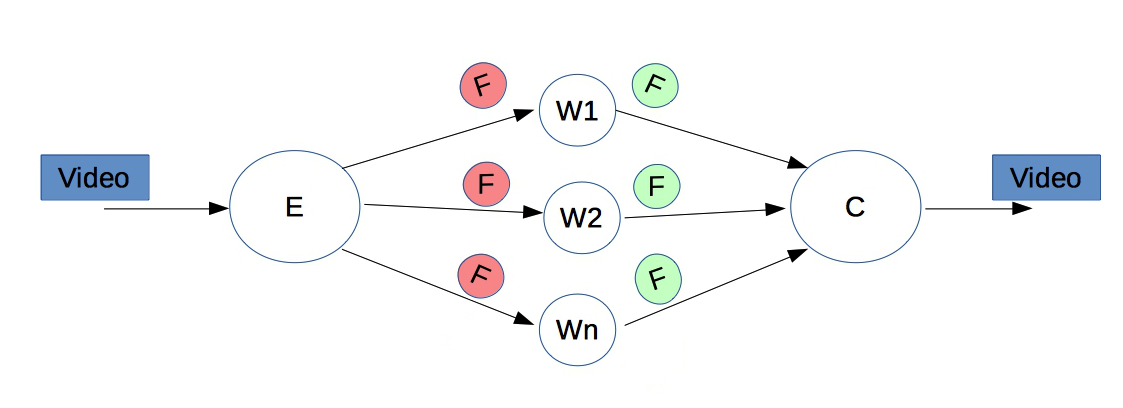
\includegraphics[scale=.32,keepaspectratio]{farm.jpg}
  \caption{Rappresentazione grafica del Modello Farm. I cerchi rossi rappresentano i frame da ridurre, quelli verdi i frame risultanti}
  \label{img:ofarm}
\end{figure}

Le scelte implementative pi\`u importanti riguardano l'implementazione del Worker e del Collector: nel primo, piuttosto che suddividere la riduzione del frame in una ulteriore farm, o mediante metodi come il ParallelFor, si \`e preferito lasciare il calcolo sequenziale all'interno del Worker, poich\`e l'eventuale overhead introdotto non \`e compensato dai risultati del calcolo parallelo in termini di tempo. Inoltre l'utilizzo di una farm all'interno di ogni worker sarebbe stato vano, poich\`e, come si vedr\`a pi\`u avanti, sebbene la riduzione del tempo d'esecuzione dei Workers porti ad una miglioria nel tempo di esecuzione totale, il tempo totale d'esecuzione \`e limitato dal tempo di esecuzione del Collector, fortemente legato dalla scrittura su file di ogni singolo frame.
\\Un'alternativa sarebbe potuta essere rimuovere il collector e lasciare il compito di scrivere i frame risultanti ad ogni worker, ed il tempo di completamento, maggiormente dettato dal tempo di servizio del collector, sarebbe diminuito in proporzione al grado di parallelismo ma la scrittura su video vanificava i risultati per via della perdita di frame.
\\Per quanto concerne il Collector, il nodo \`e stato implementato come un normale nodo, ma con la differenza che colleziona i risultati dai Workers mediante il metodo \texttt{all\_gather}: tale metodo implementa una \textbf{Map} tra i Workers e il vettore di collezione, mappando uno-a-uno ogni risultato dei Workers ed il vettore. Tale metodo risulta ottimo in termini di tempo ($\sim 0.05 ms$) ma, come si vedr\`a nei prossimi paragrafi, il tempo di servizio \`e maggiorato a causa della scrittura dei frame su video.

\subsection{StreamVideo\_Threads}
L'implementazione parallela \`e per ovvi motivi differente utilizzando la libreria Thread. Il modello sviluppato \`e, come per la precedente implementazione, il Modello Farm. 
\\Dapprima si \`e provveduto a implementare gli \textit{Shared Object}, dei contenitori utilizzati per scambiare informazioni tra i nodi della Farm: tra Emitter e Worker gli scambi avvengono mediante la \textit{SharedQueue}, una Queue con metodi \textit{push} e \textit{pop} regolati da \textit{mutex} e \textit{condition\_variable}; tra Worker e Collector gli scambi avvengono tra una \textit{SharedMap}, costruita per preservare l'ordinamento. 
\\La classe principale \`e \textit{StreamVideo}, la quale implementa al suo interno, oltre i classici Emitter, Worker, Collector, i metodi per l'esecuzione dei threads. La classe \`e rappresentata nell'algoritmo mostrato in Codice 2. 

\begin{lstlisting}[backgroundcolor=\color{White}, caption={Pseudo-code StreamVideo\_Threads}, mathescape=true] 
input: Video V, int ray, int numthreads
output: Video W
SharedQueue em-to-wor
SharedMap   wor-to-col
emitter( Video V ){
	foreach Frame  $f^{m \times n} \in V$
	em-to-wor.push(f)
}
worker( int ray ){
	while( frame = em-to-wor.pop() )
		//process frame
		wor-to-col.push(frame, pos)
}
collector( Video W ){
	while( frame = wor-to-col.pop() )
		W.write( frame )
}
create and run( int numthreads ){
	thread e( emitter )
	e.join()
	for( i = 0; i < numthreads; i++ )
		thread w( worker ))
		w.join()
	thread c( collector )
	c.join() 
}
\end{lstlisting}


\section{Valutazione delle performance}
Al fine di valutare le performance di calcolo sono stati definiti modelli analitici, in seguito confrontati con le rilevazioni su una macchina target. 
\\Le rilevazioni son state fatte mediante l'utilizzo del metodo \texttt{gettimeofday} incluso nella classe Unix \texttt{sys/tyme.h}. 
\\La macchina su cui son stati fatti i test \`e \textit{titanic.di.unipi.it} con due processori AMD Opteron 6176 a 12 cores. Il compilatore in uso \`e \texttt{GCC 4.9}.
\\Tutti i test sono realizzati utilizzando il file video \texttt{WarIsOver.avi}, contenente 250 frames e incluso nel software.

\subsection{Performance}
Nella valutazione delle performance si \`e tenuto conto di diverse misure: il Tempo di Completamento, lo SpeedUp, l'Efficiency e la Scalability.
% Il \textit{Tempo di Completamento} del modello misura il tempo totale d'esecuzione dell'applicazione, ed \`e stimato mediante la formula
% \begin{center}$T_{C}(n) = T_{emit} + \frac{T_{work}}{n} + T_{coll}$\end{center}
% dove $T_{emit}$,$T_{work}$ e $T_{coll}$ sono rispettivamente i tempi per suddividere il video in frames, processare un frame e creare un nuovo video. 
% \\Lo \textit{SpeedUp} misura la bont\`a della parallelizzazione rispetto alla miglior esecuzione sequenziale, ed \`e stimato mediante la formula
% \begin{center}$Sp(n) =  \frac{T_{seq}}{T_{par}(n)}$\end{center}
% dove $T_{seq}$ \`e il miglior tempo di completamento sequenziale $T_{par}$ \`e il tempo d'esecuzione parallela con grado di parallelismo uguale a $n$.
% \\L'\textit{Efficiency} misura l'abili\`a dell'applicazione parallela di sfruttare al meglio le risorse disponibili, ed \`e stimata mediante la formula
% \begin{center}$e(n) =  \frac{T_{id}(n)}{T_{par}(n)}$\end{center} dove $T_{id}(n)$ \`e il tempo ideale, ossia il tempo sequenziale diviso il grado di parallelismo
% \\La \textit{Scalability} misura l'efficienza dell'applicazione parallela nel raggiungere le migliori performance con alto grado di parallelismo, ed \`e stimata mediante la formula
% \begin{center} $Sc(n) = \frac{T_{par}(1)}{T_{par}(n)}$ \end{center}
% \\Tale misura \`e stata utilizzata non solo per la misura delle performance, ma anche per capire se era conveniente indrodurre modelli aggiuntivi al codice, come una OFarm che si occupi di processare in parallelo ogni singolo frame e/o utilizzare modelli di Data Parallelism come Parallel For. In entrambi i casi, i risultati hanno guidato la scelta su un'implementazione semplice, poich\`e, ad esempio, con l'uso del Parallel For, il tempo di esecuzione quadruplicava.
\\Come \`e presumibile immaginare, questo \`e un problema parallelo sui dati, dunque ci si aspetta che lo SpeedUp cresca proporzionalmente ed il tempo di completamento decresca al crescere del grado di parallelismo. Ci si aspetta dunque uno SpeedUp quasi lineare nel numero di Cores disponibili.
\\Si mostrano i risultati per le due implementazioni

\subsection{FastFlow}
Siano $T_{seq}$ e $T_{par}(n)$ rispettivamente il Completion Time dell'applicazione sequenziale e di quella parallela con grado di parallelismo $n$. L'esecuzione dello script \texttt{GetTimesAndPlots.sh} permette di stimare $T_{seq} \simeq 39.221 sec$ e $T_{par}(n)$ come riportato nella tabella \ref{fftc}.

\begin{table}[!htbp]
\centering
\caption{$T_{par}(n)$ FastFlow}
\label{fftc}
\begin{tabular}{c c c c c c c c c c c }
$n$ & 1 & 2 & 3 & 4 & 5 & 6 & 7 & 8 & 9 & 10   \\ \hline
 & 36.134 & 18.383 & 12.425 & 9.967 & 9.679 & 9.518 & 9.556 & 9.622 & 9.537 & 9.317
   \\ \\
11 & 12 & 13 & 14 & 15 & 1617 & 18 & 19 & 20 \\ \hline
9.246 & 9.424 & 9.255 & 9.149 & 9.193 & 9.144 & 9.247 & 9.253 & 9.240 & 9.268
  \\ \\
21 & 22 & 23 & 24 \\ \hline
9.137 & 9.121 & 11.207 & 10.955
\end{tabular}
\end{table}
Le performance per lo Speedup, indicato con $sp(n)$, sono riportate nella tabella \ref{ffsp}.
\begin{table}[!htbp]
\centering
\caption{$sp(n)$ FastFlow}
\label{ffsp}
\begin{tabular}{c c c c c c c c c c c }
$n$ & 1 & 2 & 3 & 4 & 5 & 6 & 7 & 8 & 9 & 10   \\ \hline
 & 1.085 & 2.133 & 3.156 & 3.934 & 4.051 & 4.120 & 4.104 & 4.075 & 4.112 & 4.209
  \\ \\
11 & 12 & 13 & 14 & 15 & 16 & 17 & 18 & 19 & 20 \\ \hline
4.241 & 4.161 & 4.237 &4.286 & 4.266 & 4.289 & 4.241 & 4.238 & 4.244 & 4.231\\
21 & 22 & 23 & 24 \\ \hline
4.292 & 4.299 & 3.499 & 3.579
\end{tabular}
\end{table}
Le performance per l'Efficency, indicato con $e(n)$, sono riportate nella tabella \ref{ffef}.
\begin{table}[!htbp]
\centering
\caption{$e(n)$ FastFlow}
\label{ffef}
\begin{tabular}{c c c c c c c c c c c }
$n$ & 1 & 2 & 3 & 4 & 5 & 6 & 7 & 8 & 9 & 10   \\ \hline
& 1.085 & 1.067 & 1.052 & 0.984 & 0.810 & 0.687 & 0.586 & 0.510 & 0.457 & 0.421
  \\ \\
11 & 12 & 13 & 14 & 15 & 16 &17 & 18 & 19 & 20 \\ \hline
0.386 & 0.347 & 0.326 & 0.306 & 0.284 & 0.268 & 0.249 & 0.235 & 0.223 & 0.212
  \\ \\
21 & 22 & 23 & 24 \\ \hline
0.204 & 0.195 & 0.152 & 0.149
\end{tabular}
\end{table}
Le performance per la Scalability, indicato con $sc(n)$, sono riportate nella tabella \ref{ffsc}.
\begin{table}[!htbp]
\centering
\caption{$sc(n)$ FastFlow}
\label{ffsc}
\begin{tabular}{c c c c c c c c c c c }
$n$ & 1 & 2 & 3 & 4 & 5 & 6 & 7 & 8 & 9 & 10   \\ \hline
& 1.000 & 1.965 & 2.908 & 3.625 & 3.733 & 3.796 & 3.781 & 3.755 & 3.788 & 3.878 
 \\ \\
11 & 12 & 13 & 14 & 15 & 16 &17 & 18 & 19 & 20 \\ \hline
3.907 & 3.833 & 3.903 & 3.949 & 3.930 & 3.951 & 3.907 & 3.904 & 3.910 & 3.898
 \\ \\
21 & 22 & 23 & 24 \\ \hline
3.954 & 3.961 & 3.223 & 3.298
\end{tabular}
\end{table}

Si riportano, per immediatezza visiva, le precedenti tabelle su grafico nella figura \ref{img:plotsff}.
\begin{figure}[!htbp]
\begin{subfigure}{.55\textwidth}
  \centering
  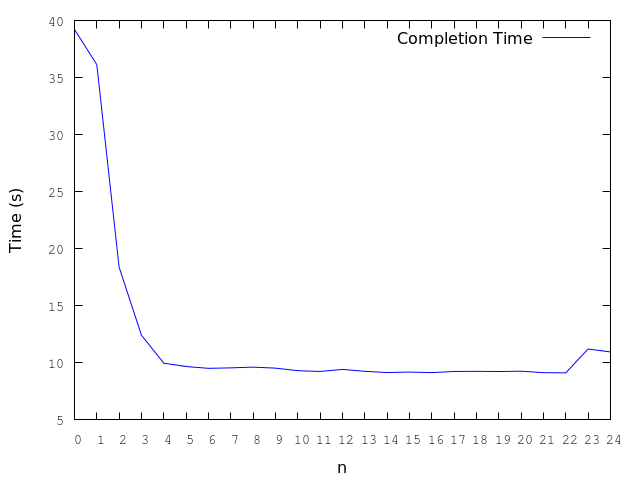
\includegraphics[scale=.35,keepaspectratio]{ff_tc.png}
  \caption{$T_{par}(n)$}
  \label{fig:tisc}
\end{subfigure} 
\begin{subfigure}{.55\textwidth}
  \centering
  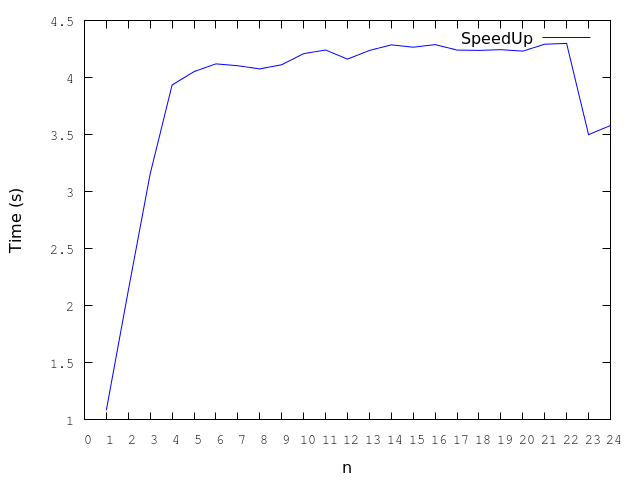
\includegraphics[scale=.35,keepaspectratio]{ff_sp.png}
  \caption{$sp(n)$}
  \label{fig:ftsec}
\end{subfigure}
\begin{subfigure}{.55\textwidth}
  \centering
  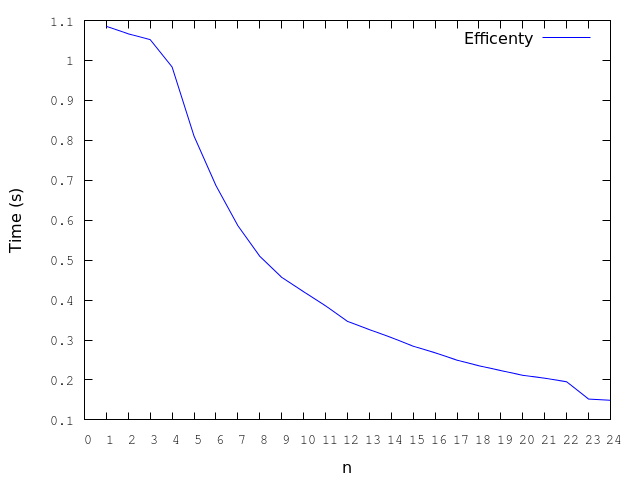
\includegraphics[scale=.35,keepaspectratio]{ff_ef.png}
  \caption{$e(n)$}
  \label{fig:lsec}
\end{subfigure}
\begin{subfigure}{.55\textwidth}
  \centering
  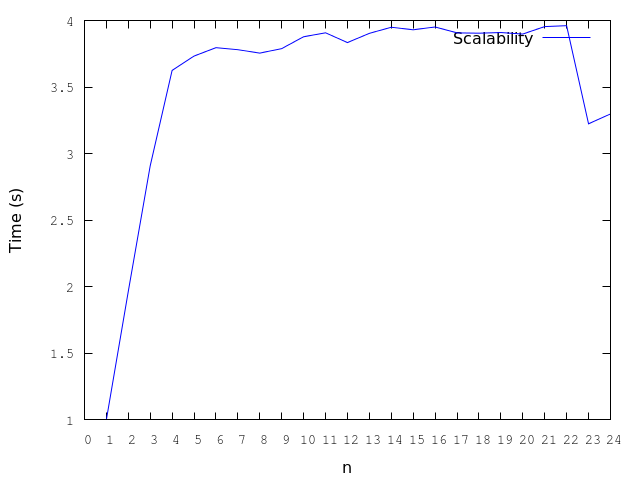
\includegraphics[scale=.35,keepaspectratio]{ff_sc.png}
  \caption{$sc(n)$}
  \label{fig:cacc}
\end{subfigure}
\caption{Performance implementazione FastFlow}
\label{img:plotsff}
\end{figure}

Come si pu\`o notare anche dai grafici, il Tempo di Completamento decresce vertiginosamente fino ad un grado di parallelismo uguale a 5, questo perch\`e il Tempo di Completamento \`e fortemente vincolato al Tempo dei Workers i quali processano i dati e poi inviano al Collector. Dunque bisogna attendere almeno che tutti i Workers abbiano processato tutti i dati, ma sopratutto bisogna attendere che il Collector scriva i risultati sul video, ed il Tempo del Collector, sebbene il metodo \texttt{all\_gather} \`e super efficiente, risulta limitato dalla scrittura su video, la quale \`e molto lenta: 1 frame $\sim 44ms \times 250$, 2 frames $\sim 94ms \times 125$, 10 frames $\sim 432ms \times 25$, 24 frames $\sim 936ms \times 11$, che appunto, quest'ultima, supera i 10sec. Il Tempo dei Workers pu\`o dunque decrescere, ma sar\`a fortemente sovralimitato dal tempo del Collector. Sia lo Speedup, sia l'Efficiency e la Scalability, sono fortemente legati da questi fattori, e i loro grafici lo confermano. In fig.\ref{img:evidence} si nota appunto il confronto tra Tempo dei Workers (mediato sul numero degli stessi) e tempo del Collector.
\begin{figure}[!htbp]
\begin{subfigure}{.55\textwidth}
  \centering
  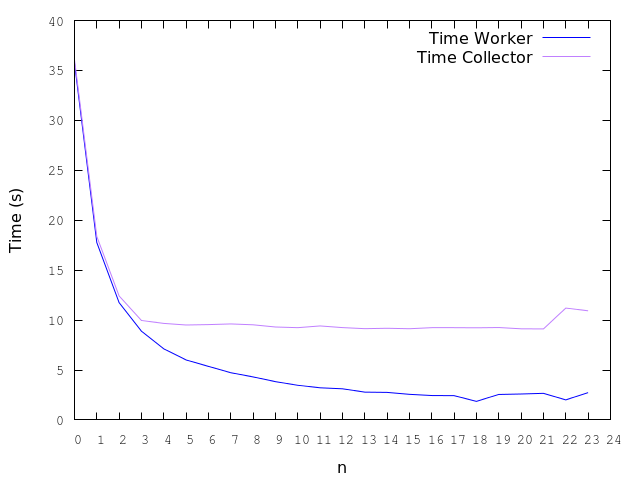
\includegraphics[scale=.55,keepaspectratio]{ff_evidence_time.png}
  \caption{}
  \label{fig:tisc}
\end{subfigure} 
\caption{Confronto fra Collector Time e Worker Time}
\label{img:evidence}
\end{figure}

\subsection{Threads C++11}
L'esecuzione dello script \texttt{GetTimesAndPlots.sh} permette di stimare $T_{seq} \simeq 39.221$ e $T_{par}(n)$ come riportato nella tabella \ref{fftc1}.

\begin{table}[!htbp]
\centering
\caption{$T_{par}(n)$ Threads}
\label{fftc1}
\begin{tabular}{c c c c c c c c c c c }
$n$ & 1 & 2 & 3 & 4 & 5 & 6 & 7 & 8 & 9 & 10   \\ \hline
& 39.344 & 21.327  & 15.401 &  12.578 & 10.478 & 9.486 & 8.632 & 7.710 & 7.193 & 6.970 
  \\ \\
11 & 12 & 13 & 14 & 15 & 1617 & 18 & 19 & 20 \\ \hline
6.888 & 6.219 & 6.046 & 5.891 & 5.813 & 5.636 & 5.722 & 5.435 & 5.269  & 5.123 
  \\ \\
21 & 22 & 23 & 24 \\ \hline
 4.898 & 4.909 & 4.771 & 4.777 
\end{tabular}
\end{table}
Le performance per lo Speedup, indicato con $sp(n)$, sono riportate nella tabella \ref{ffsp1}.
\begin{table}[!htbp]
\centering
\caption{$sp(n)$ Threads}
\label{ffsp1}
\begin{tabular}{c c c c c c c c c c c }
$n$ & 1 & 2 & 3 & 4 & 5 & 6 & 7 & 8 & 9 & 10   \\ \hline
& .996 & 1.838 & 2.546 & 3.118 & 3.743 & 4.134 & 4.543 & 5.087 & 5.452 & 5.627
  \\ \\
11 & 12 & 13 & 14 & 15 & 16 & 17 & 18 & 19 & 20 \\ \hline
5.693 & 6.306 & 6.486 & 6.657 & 6.746 & 6.959 & 6.8540 & 7.216 & 7.442 & 7.655
  \\ \\
21 & 22 & 23 & 24 \\ \hline
8.006 & 7.988 & 8.219 & 8.209
\end{tabular}
\end{table}

Le performance per l'Efficency, indicato con $e(n)$, sono riportate nella tabella \ref{ffef1}.
\begin{table}[!htbp]
\centering
\caption{$e(n)$ Threads}
\label{ffef1}
\begin{tabular}{c c c c c c c c c c c }
$n$ & 1 & 2 & 3 & 4 & 5 & 6 & 7 & 8 & 9 & 10   \\ \hline
& .996 & .919 & .848 & .779 & .748 & .689 & .649 & .635 & .605 & .562 
  \\ \\
11 & 12 & 13 & 14 & 15 & 16 & 17 & 18 & 19 & 20 \\ \hline
.517 & .525 & .498 & .475 & .449 & .434 & .403 & .400 & .391 & .382
  \\ \\
21 & 22 & 23 & 24 \\ \hline
.381 & .363 & .357 & .342
\end{tabular}
\end{table}

Le performance per la Scalability, indicato con $sc(n)$, sono riportate nella tabella \ref{ffsc1}.
\begin{table}[!htbp]
\centering
\caption{$sc(n)$ Threads}
\label{ffsc1}
\begin{tabular}{c c c c c c c c c c c }
$n$ & 1 & 2 & 3 & 4 & 5 & 6 & 7 & 8 & 9 & 10   \\ \hline
& 1.000 & 1.844 & 2.554 & 3.127 & 3.754 & 4.147 & 4.557 & 5.103 & 5.469 & 5.644
 \\ \\
11 & 12 & 13 & 14 & 15 & 16 & 17 & 18 & 19 & 20 \\ \hline
5.711 & 6.326 & 6.507 & 6.678 & 6.767 & 6.980 & 6.875 & 7.238 & 7.466 & 7.679
 \\ \\
21 & 22 & 23 & 24 \\ \hline
8.031 & 8.013 & 8.244 & 8.235
\end{tabular}
\end{table}

Si riportano, per immediatezza visiva, le precedenti tabelle su grafico nella figura \ref{img:plotsth}.
\begin{figure}[!htbp]
\begin{subfigure}{.55\textwidth}
  \centering
  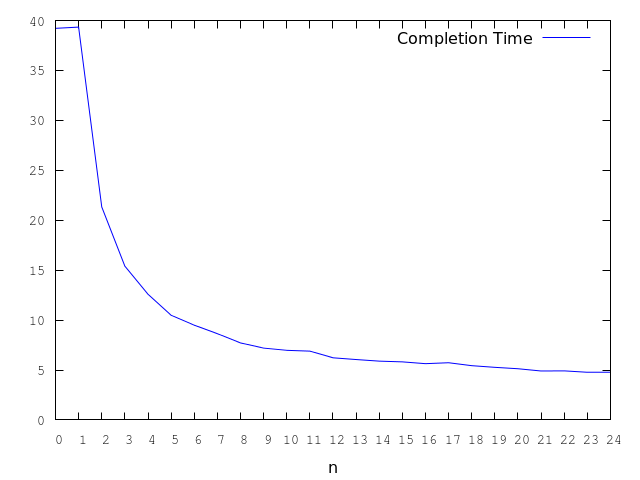
\includegraphics[scale=.35,keepaspectratio]{th_tc.png}
  \caption{$T_{par}(n)$}
  \label{fig:tisc}
\end{subfigure} 
\begin{subfigure}{.55\textwidth}
  \centering
  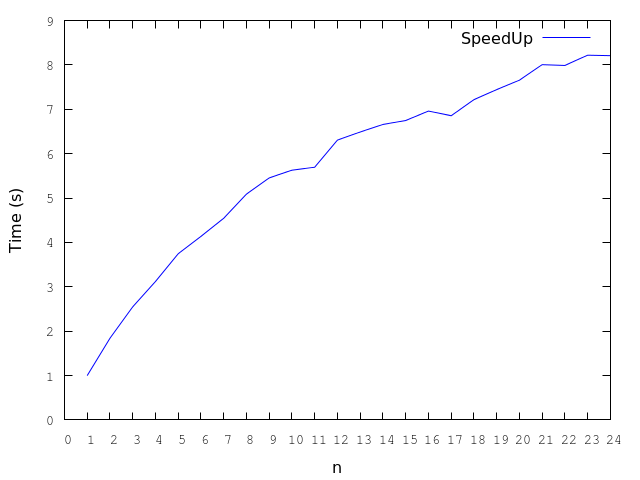
\includegraphics[scale=.35,keepaspectratio]{th_sp.png}
  \caption{$sp(n)$}
  \label{fig:ftsec}
\end{subfigure}
\begin{subfigure}{.55\textwidth}
  \centering
  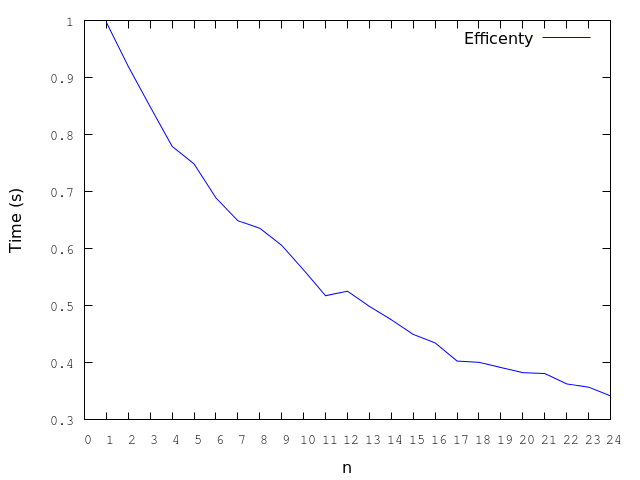
\includegraphics[scale=.35,keepaspectratio]{th_ef.png}
  \caption{$e(n)$}
  \label{fig:lsec}
\end{subfigure}
\begin{subfigure}{.55\textwidth}
  \centering
  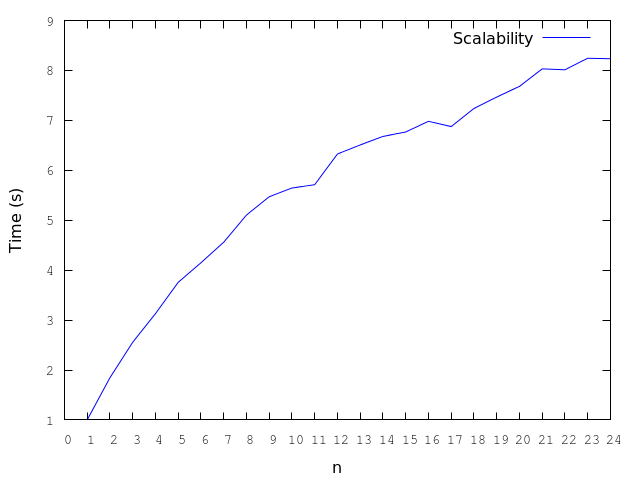
\includegraphics[scale=.35,keepaspectratio]{th_sc.png}
  \caption{$sc(n)$}
  \label{fig:cacc}
\end{subfigure}
\caption{Performance implementazione Threads C++11}
\label{img:plotsth}
\end{figure}

Come si pu\`o notare dai grafici, lo Speedup cresce in maniera lineare al grado di parallelismo, cos\`i come l'efficienza e la scalabilit\`a, il che fa presumere che l'implementazione con Threads di C++11 raggiunge prestazioni migliori.
\\Si riportano, per competezza, i grafici di entrambe le implementazioni comparate in figura \ref{img:plottot}.
\begin{figure}[!htbp]
\begin{subfigure}{.55\textwidth}
  \centering
  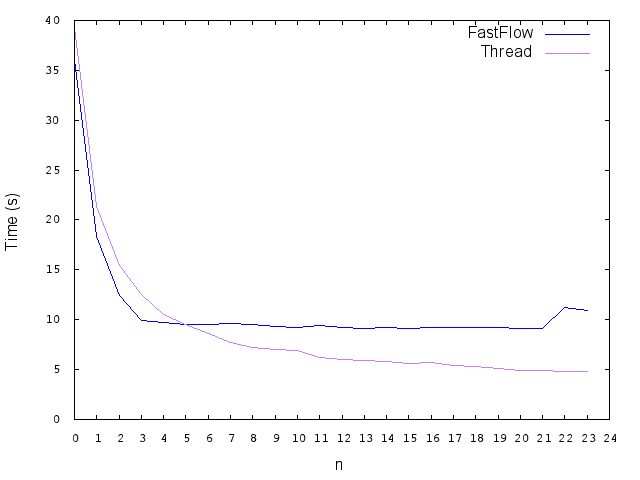
\includegraphics[scale=.35,keepaspectratio]{tc.png}
  \caption{$T_{par}(n)$}
  \label{fig:tisc}
\end{subfigure} 
\begin{subfigure}{.55\textwidth}
  \centering
  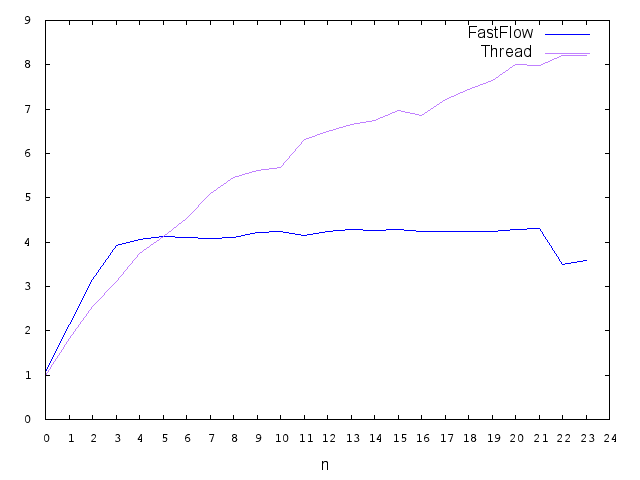
\includegraphics[scale=.35,keepaspectratio]{sp.png}
  \caption{$sp(n)$}
  \label{fig:ftsec}
\end{subfigure}
\begin{subfigure}{.55\textwidth}
  \centering
  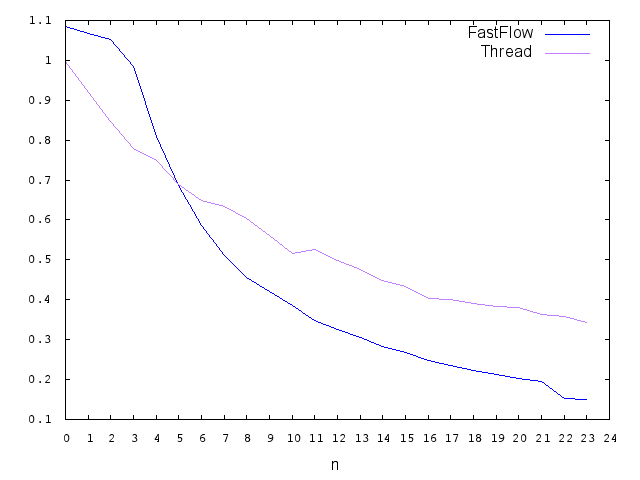
\includegraphics[scale=.35,keepaspectratio]{ef.png}
  \caption{$e(n)$}
  \label{fig:lsec}
\end{subfigure}
\begin{subfigure}{.55\textwidth}
  \centering
  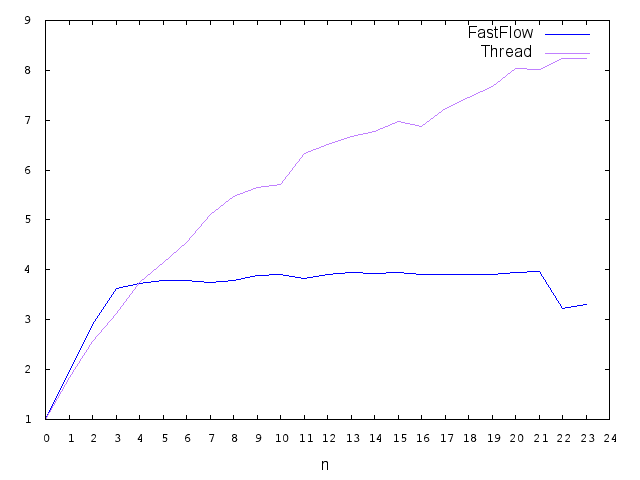
\includegraphics[scale=.35,keepaspectratio]{sc.png}
  \caption{$sc(n)$}
  \label{fig:cacc}
\end{subfigure}
\caption{Performance delle due implementazioni}
\label{img:plottot}
\end{figure}

\newpage
\appendix
\section{Manuale d'uso} \label{App:AppendixA}
Una copia del Software \`e presente nella macchina \texttt{titanic.di.unipi.it}, nella directory \texttt{/home/idini/SPM/}
\subsection{Makefile}
Prima di utilizzare il software \`e necessario compilarlo, recandosi all'interno della directory dove esso \`e contenuto e da terminale eseguire il comando:
\begin{lstlisting}[language=bash]
  $ make
\end{lstlisting}
Esso compiler\`a i tre file contenuti all'interno della directory stessa: 
\begin{description}
\item[Sequential.cpp] \`e il file contenente l'implementazione sequenziale
\item[StreamVideo\_FastFlow.cpp] \`e il file contenente l'implementazione parallela utilizzando la libreria FastFLow
\item[StreamVideo\_Threads.cpp] \`e il file contenente l'implementazione parallela utilizzando la libreria standard Threads C++11
\end{description}
Al fine di compilare il software in maniera efficiente e compatibile \`e necessario aver sulla propria macchina una versione di GCC uguale o superiore a 4.8. Per visualizzare la versione del compilatore installata sulla propria macchina, eseguire 
\begin{lstlisting}[language=bash]
  $ gcc --version
\end{lstlisting}
o
\begin{lstlisting}[language=bash]
  $ gcc -dumpversion
\end{lstlisting}

\subsection{Eseguibili}
Gli eseguibili risultanti dalla compilazione sono:
\begin{description}
\item[Sequential] il quale accetta in input 3 parametri: \textbf{filevideo.avi} \textbf{ray} \textbf{outputvideo.avi}
\item[StreamVideo\_FastFlow] il quale accetta in input 4 parametri: \textbf{filevideo.avi} \textbf{ray} \textbf{outputvideo.avi} \textbf{filevideo.avi} \textbf{num\_threads} 
\item[StreamVideo\_Threads] il quale accetta in input 4 parametri: \textbf{filevideo.avi} \textbf{ray} \textbf{outputvideo.avi} \textbf{num\_threads} 
\end{description}

\subsection{Script}
Sono forniti inoltre degli script in \texttt{Bash}:
\begin{description}
  \item[GetTimesAndPlots.sh] compila, se non \`e stato ancora fatto, il codice elencato precedentemente, calcola il \textit{Tempo di Completamento} per l'implementazione sequenziale e \textit{Tempo di Completamento}, \textit{Scalabilit\`a}, \textit{Efficienza} e \textit{Speedup} per ognuna delle due implementazioni parallele
\end{description}
I plot, dopo l'esecuzione di quest'ultimo, si possono trovare all'interno della directory \texttt{plot/}, mentre i tempi si possono trovare all'interno della cartella \texttt{tmp/}.

\subsection{Licenza}
Tutto il codice sorgente scritto viene rilasciato sotto licenza Gnu GPL - General Public Licence versione 3, ognuno \`e libero di modificare e di distribuire il codice sorgente entro i termini di tale licenza. Tale licenza pu\`o essere consultata all’indirizzo: \url{http://www.gnu.org/copyleft/gpl.html}

\\Copyright \textcopyright  2016  Maurizio Idini.

\\Permission is granted to copy, distribute and/or modify this document
under the terms of the GNU Free Documentation License, Version 1.3
or any later version published by the Free Software Foundation;
with no Invariant Sections, no Front-Cover Texts, and no Back-Cover Texts.

\\Per qualsiasi problema e/o quesito \`e possibile contattare lo sviluppatore all'indirizzo e-mail maurizio.idini [at] gmail.com

\end{document}

